\documentclass[a4paper,10pt]{article}


\usepackage{t1enc}
\usepackage{linguex}
\usepackage{harvard}
\usepackage{graphicx}
\usepackage{amsmath}
\usepackage{amssymb}
\usepackage{graphicx}
\usepackage{tikz}
\usetikzlibrary{arrows,automata}
\usepackage{subfigure}
\usepackage{qtree}
%\usepackage{hyperref}




\bibliographystyle{diss}

%opening
\title{Results K2s}
\author{}



\newtheorem{hypothese}{Hypothesis}
\newtheorem{Def}{Definition}
\newtheorem{Prop}{Proposition}
\newtheorem{Example}{Example}

\begin{document}

\maketitle

\begin{abstract}

\end{abstract}

\section{Results}
The judgments obtained for the four target conditions are depicted   in Figure \ref{fig:JudgmentsK2}.  We coded the judgments as {\it literal}, {\it global} or {\it local} if they were as expected under one of these readings and as {\it error} if not. The distribution of readings as coded by us is presented in Figure \ref{fig:ReadingsExp1}. Participants mostly gave judgments indicating literal or local readings. Judgments compatible with a global reading were seldomly obtained. In the All-Some conditions participants made hardly any errors, whereas the amount of errors was slightly greater in the Exactly-One-Some conditions.

\begin{figure}[h]
\centering
\subfigure[All-Some accented]{
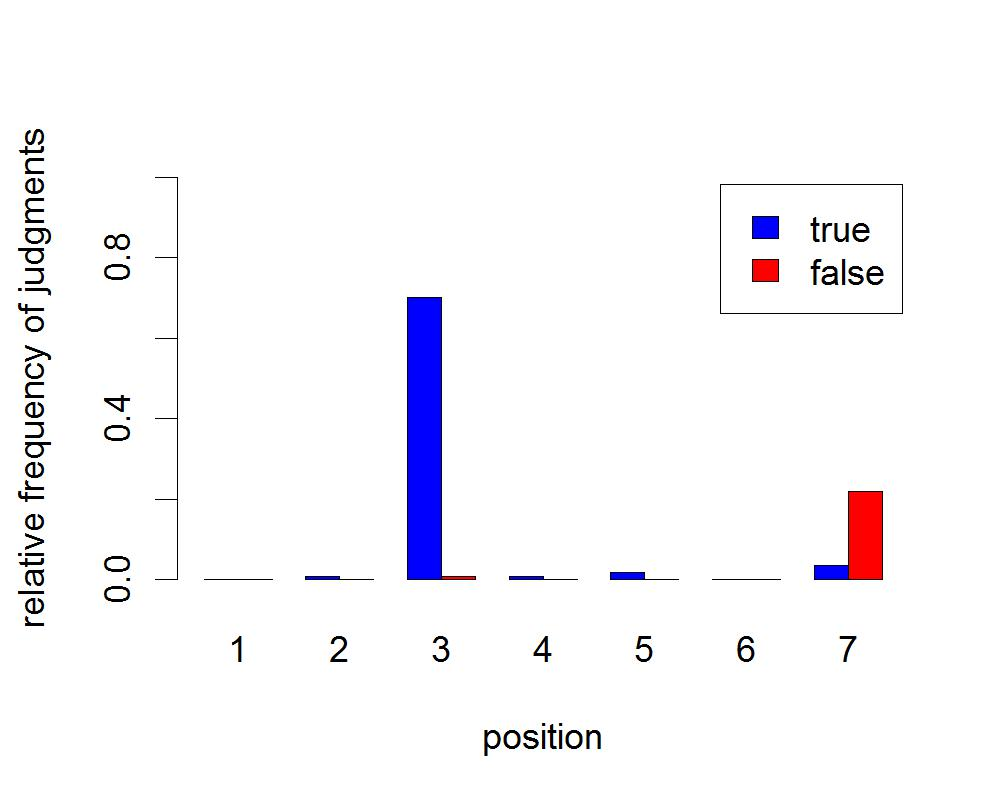
\includegraphics[width=5cm]{graph_AE_AKZ.jpg}
\label{fig:ReadingsAE}
}
\subfigure[All-Some neutral]{
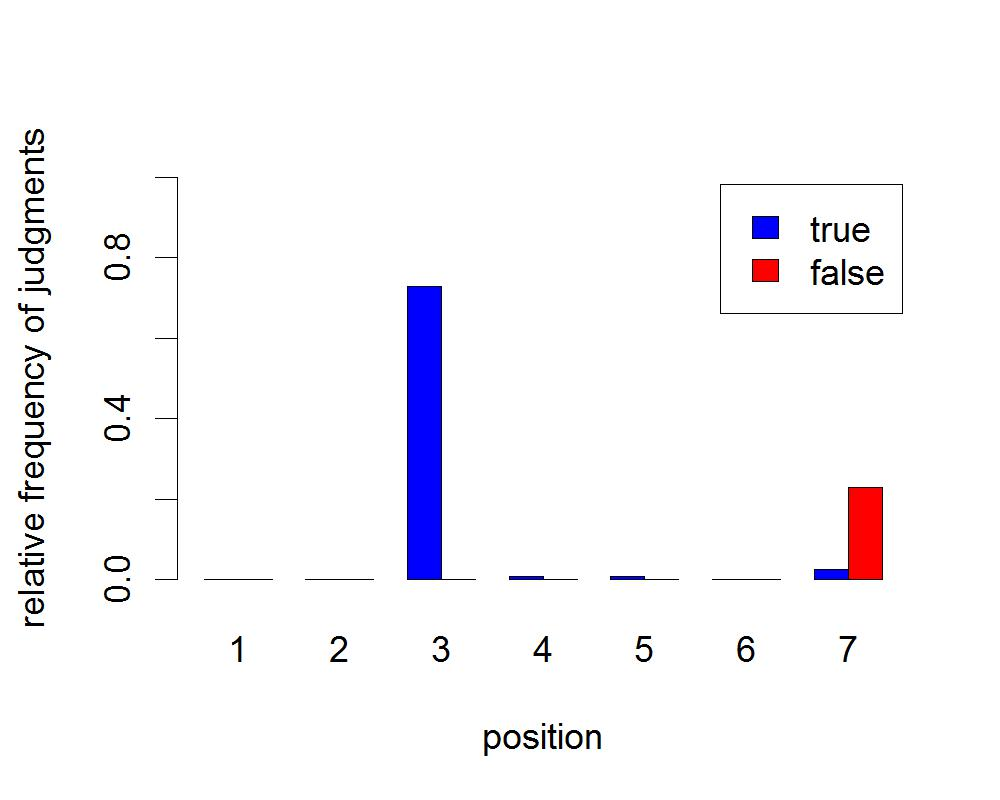
\includegraphics[width=5cm]{graph_AE_NTR.jpg}
\label{fig:ReadingsGE}
}
\subfigure[Exactly-One-Some accented]{
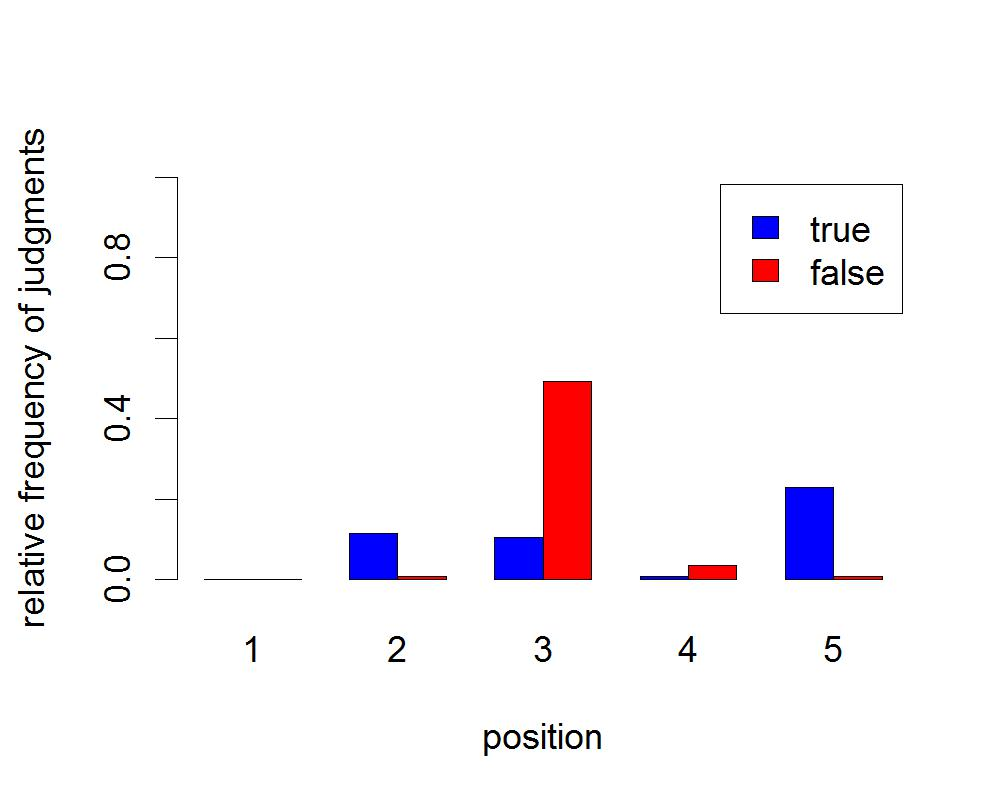
\includegraphics[width=5cm]{graph_GE_AKZ.jpg}
\label{fig:ReadingsAE}
}
\subfigure[Exactly-One-Some neutral]{
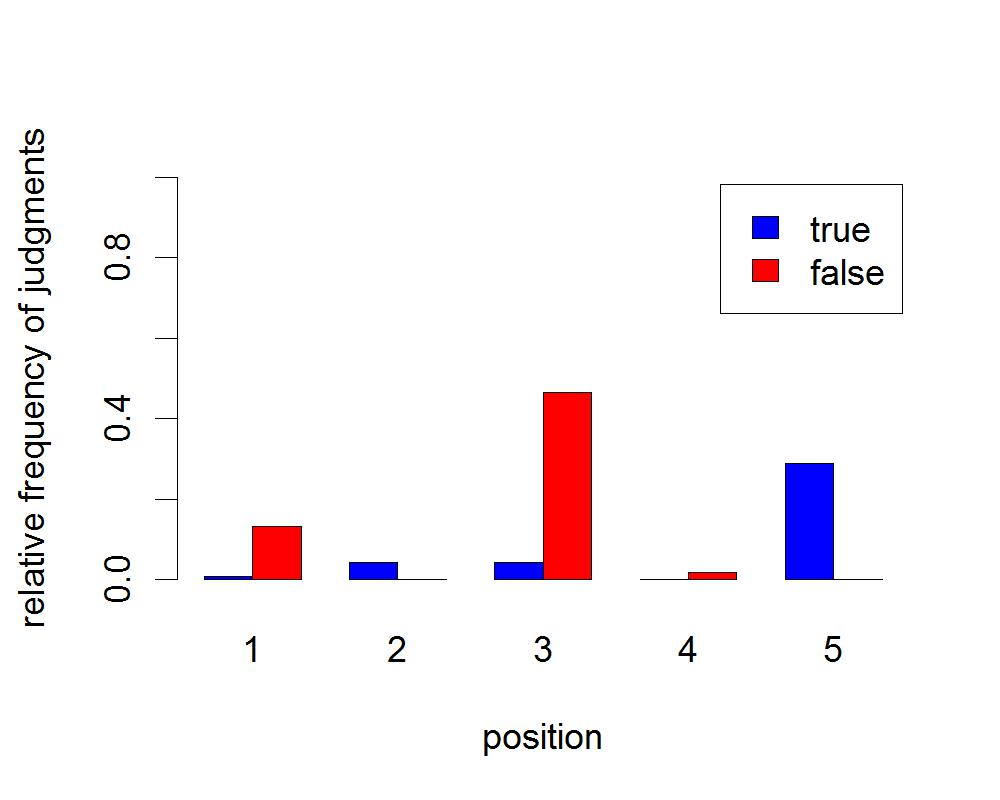
\includegraphics[width=5cm]{graph_GE_NTR.jpg}
\label{fig:ReadingsGE}
}

\caption[Optional caption for list of figures]{Judgments for the four target conditions in Experiment 1. Relative frequency of yes/no-judgments is plotted against the position within the trial. In the All-Some conditions there were seven positions. On the third position a yes-judgment corresponded to a literal reading, while on the fith position a yes-judgment corresponded to a global reading.  A no-judgment on the seventh position was only consistent with a local reading. The Exactly-One-Some conditions had five positions. No- judgments on positions two and three corresponded to global and literal readings, respectively. A yes-judgment on the last segment  corresponded to a local reading. }
\label{fig:JudgmentsK2}
\end{figure}

In the All-Some conditions  (see Figure \ref{fig:ReadingsAE}) judgments were consistent with literal readings in 65.0\% of the trials with neutral prosody and in 67.5\% of the trials with accented prosody. The number of global readings was very low, with 1.6\% of the neutral and 0.8\% of the accented trials. Judgments indicating local readings were given in 22.0\% of both the neutral and accented trials. In the Exactly-One-Some conditions (see Figure \ref{fig:ReadingsGE}) judgments consistent with literal readings were given in 47.2\% and 44.7\% of the trials with neutral and accented prosody, respectively. Global readings were observed in 0.8\% of the trials in both the neutral and the accented condition. Judgments indicating local readings were given in 22.8\% of the neutral and 27.6\% of the accented trials.

In order to test wether local readings exist we tested whether the number of local responses in each condition was higher than expected by chance. Local responses had to be given on the last position in each trial. If local readings didn't exist we would expect participants, who reached the last position (ie. who did not abort the trial prior to the last position) to give local judgments not more often than expected by chance. On the last position two responses were possible. One was compatible with a local reading the other was not. Therefore, we would expect 50\% local responses by chance. As it turns out  local responses were given significantly more often than 50\% in all target conditions (all Bonferoni corrected p<.05). Note that this finding cannot be explained by some kind of general response bias on the last position since local readings required a yes-judgment in the Exactly-One-Some conditions but a no-judgment in the All-Some conditions.

In order to test whether accentuation or the quantifier has an influence on the distribution of readings, log-liner models were computed (see Schepers 2003). The factors {\it Reading}, {\it Accentuation} and {\it Quantifier} were included in these models. Two variants of these models were computed.  In the first, the factor {\it Item} was added to the above mentioned. In the latter {\it Participants} was included as a factor. Inclusion of these two factors allowed us to test whether the distribution of readings was identical accros items and participants. We report log-likelihood ratio Chi-squares ($LRCS_1$ and $LRCS_2$), degrees of freedom ($df_1$, $df_2$) and significance levels ($p_1$ and $p_2$).

Unsurprisingly, there was an effect of reading ($LRCS_1=364.77, df_1 = 3, p_1<.001, LRCS_2=364.77, df_2 = 3, p_1<.001,$) because overall the readings were distributed inhomogeneously (sse Figure \ref{fig:ReadingsGE}). The quantifier had an influence on the distribution of readings as revealed by a reliable interaction of {\it Reading} and {\it Quantifier} ($LRCS_1=49.32, p_1<.01,LRCS_2=32.16, p_1<.01,$). Looking at the data  it seemed unlikely that the quantifier affected the amount of local readings. We suspected that this interaction was due to the higher number of errors and lower number of literal readings in the Exactly-One-Some conditions as compared with the All-Some conditions. A difference in the distribution of judgment types between participants was revealed by a reliable interaction of {\it Reading} and {\it Participant} ($LRCS_1=487.70, p_1<.01$). We were interested in whether this effect was due to some of the participants being more likely to choose literal readings than others. Finally, there was a three-way interaction of {\it Participants}, {\it Construction} and {\it Reading} ($LRCS_1, = 143.92, df_1 = 117, p_1<.05$) which could stem from to the fact that some participants were more prone than others to make errors in the Exactly-One-Some conditions.  

In order to find out whether the interactions just reported affected the amount of local readings, the log-linear models were computed again with a different coding of the readings. Here,  we only considered the amount of local readings versus all other kinds of judgments. Judgments were coded as {\it local} and {\it other}. If the reported interactions affect the amount of local readings they should show up again. The  expected but irrelevant effect of {\it Reading} was again significant ($LRCS_1=134.55, df_1 = 1, p_1<.001, LRCS_2=144.64, df_2 = 1, p_1<.001,$). In addition, the interaction of {\it Participant} and {\it Reading} ($LRCS_1=487.70, p_1<.01$) as well as the three-way interaction of {\it Construction}, {\it Participant} and {\it Reading} ($LRCS_1=487.70, p_1<.01$) were significant. No other effects were significant. In particular, the interaction of {\it Construction} and {\it Reading} was not significant ($LRCS_1=2.10, p_1=.15,LRCS_2=.74, p_2=.39$).

The interaction of {\it Participant} and {\it Reading} shows that there are indeed varying preferences for local readings among German speakers. Further examination of the distribution of local readings revealed a clear pattern (see Figure \ref{fig:HistogramLocalReadingsK2}). In all four conditions, about  seven out of the 40 participants ($16\%$)  were consitently giving judgments that indicate local readings. Further, the relative frequency of local judgments per participant strongly correlated between all four conditions (all $r>.6, p<.001$). Appart from the localists about half of the participants (and 41.5\% of all participants) were consitently giving judgments that indicate literal readings. Only a minority of participants exhibited inconsistency. Reading preferences were  more clear-cut in the All-Some conditions than in the Exactly-One-Some conditions. The number of consitent litaralists was lower in the Exactly-One-Some (25.6\%) conditions as compared to the All-Some conditions (57.3\%). Also, the number of participants that showed inconsitency was higher in these conditions. However, the number of consistent localists did hardly differ between constructions.  

The three way-interaction of {\it Participant}, {\it Construction} and {\it Reading} is due to the fact that for some participants preferences for local over other readings deviated between the two construction types. These deviations were, however, not systematic to any degree. How much local preferences deviated between the two contsruction types per participant is depicted in Figure \ref{}. Most participants had exactly the same preferences in the two constructions. However, a few had a stronger and a few others a weaker preference for local readings in the Exactly-One-Some than in the All-Some conditions. Since we did not find any sytematic patterns here, we speculate that the three-way interaction is due to the Exactly-One-Some construction beeing understood non-standardly by a few participants. This speculation is plausible given the higher number of errors in the Exactly-One-Some  as compared to the All-Some conditions.   

The absence of the interaction between {\it Construction} and {\it Participant} indicates that the type of construction does not affect the amount of local readings. We assumed based on the observed distribution of judgments that the type of contsruction affected the amount of literal but not local and global readings. To further test this assumption, we also considered literal and global readings versus other judgments in separate analyses. Comparing global readings versus other judgments {\it Construction} and {\it Reading} were found to interact ($LRCS_1=42.80, df= 1, p<.001; LRCS_2=22.14, df= 1, p<.001$). Comparing global readings to other judgments no such interaction was obeserved ($LRCS_1=1.24, df= 1, p=.29, LRCS_1=.21, df= 1, p=.65$).

 

\begin{figure}[h]
\centering
\subfigure[All-Some Conditions]{
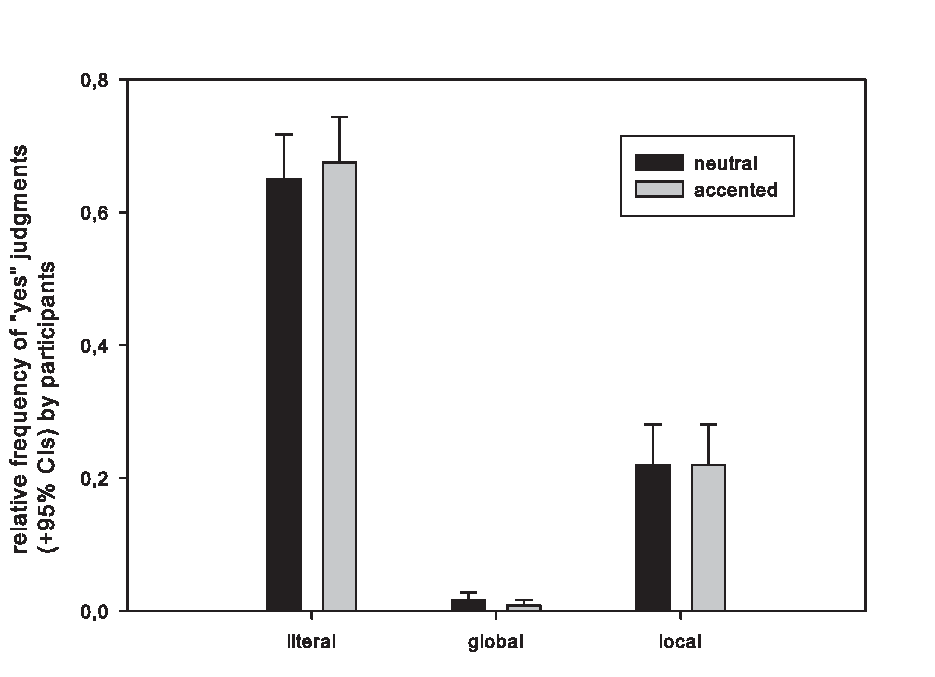
\includegraphics[width=5cm]{ReadingsAE.eps}
\label{fig:ReadingsAE}
}
\subfigure[Exactly-One-Some Conditions]{
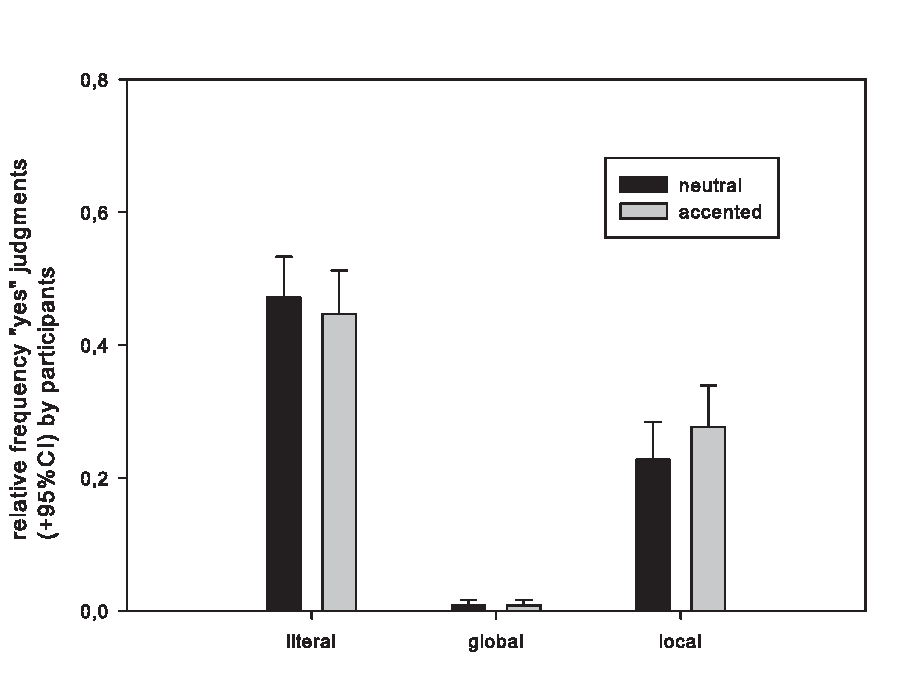
\includegraphics[width=5cm]{ReadingsGE.eps}
\label{fig:ReadingsGE}
}
\caption[Optional caption for list of figures]{Judgments}
\label{fig:ReadingsExp1}
\end{figure}

\begin{figure}[h]
\centering
\subfigure[All-Some accented]{
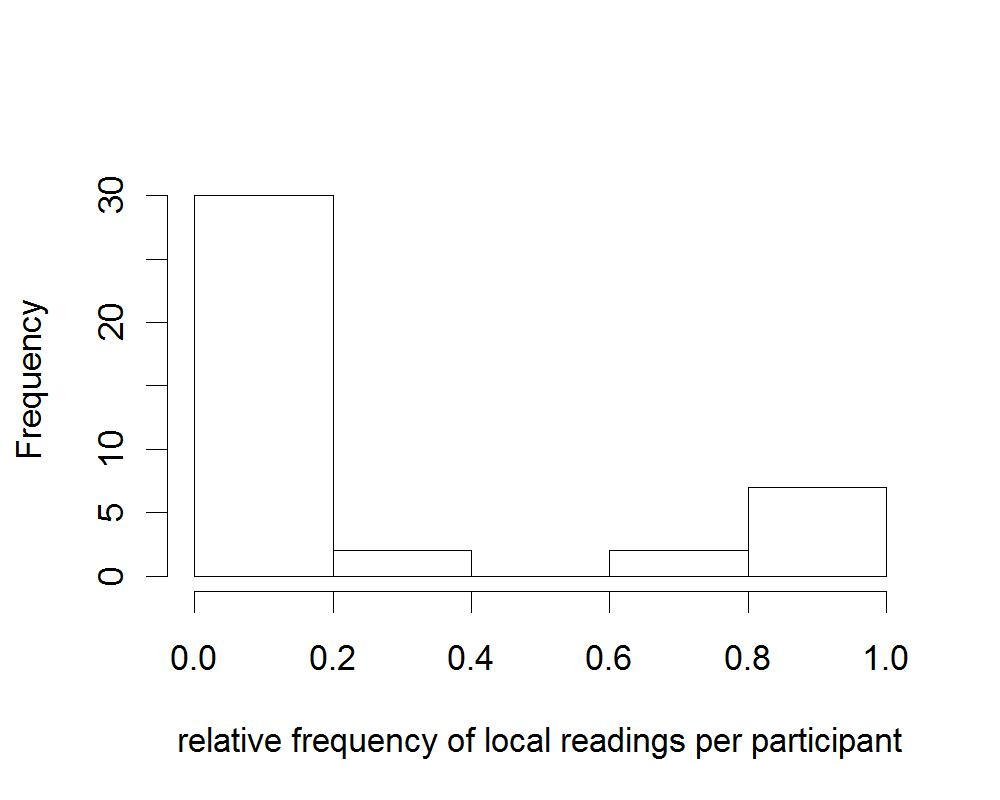
\includegraphics[width=5cm]{histLocalReadingAE_AKZ.jpg}
\label{fig:ReadingsAE}
}
\subfigure[All-Some neutral]{
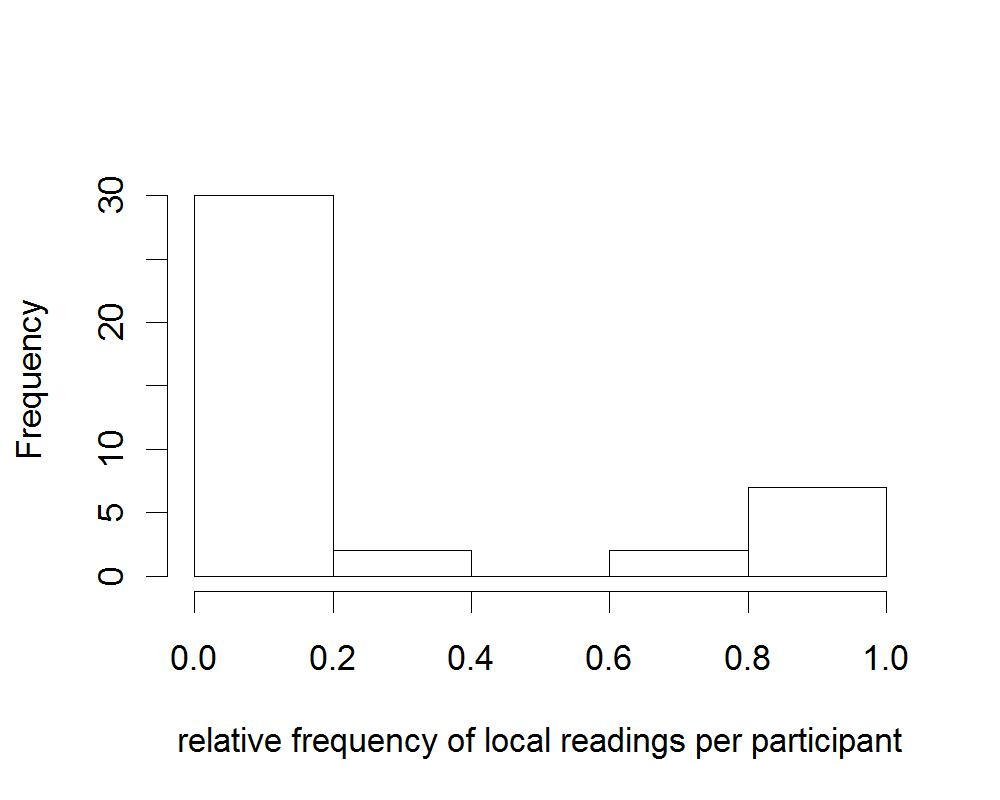
\includegraphics[width=5cm]{histLocalReadingAE_NTR.jpg}
\label{fig:ReadingsGE}
}
\subfigure[Exactly-One-Some accented]{
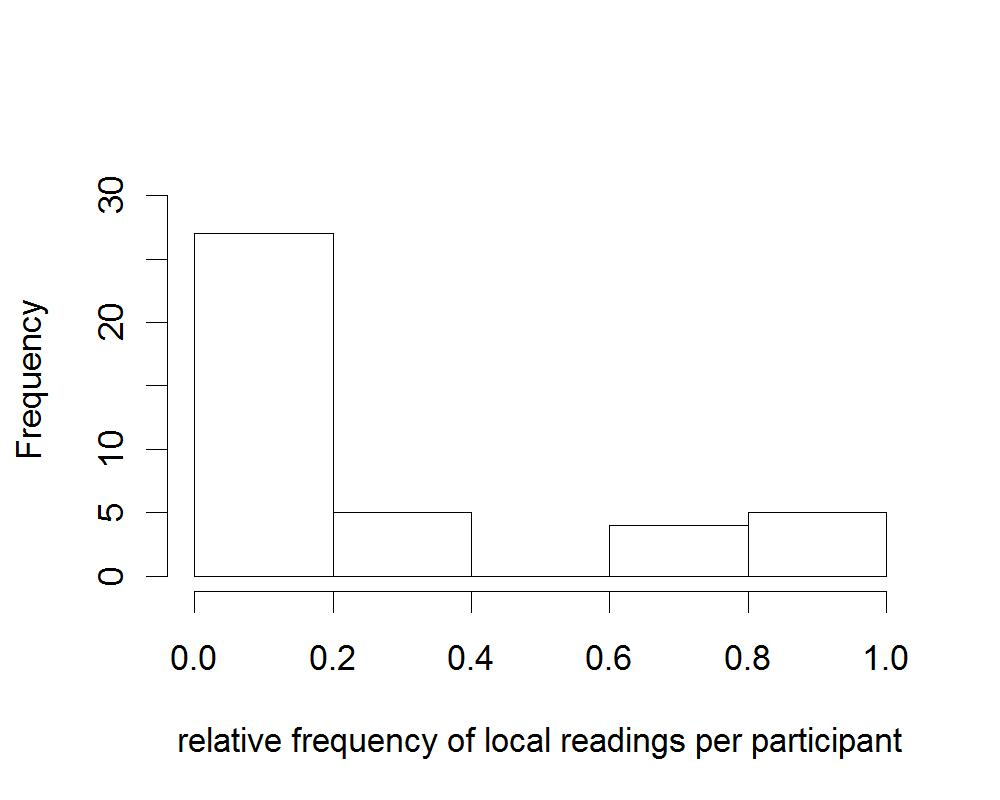
\includegraphics[width=5cm]{histLocalReadingGE_AKZ.jpg}
\label{fig:ReadingsAE}
}
\subfigure[Exactly-One-Some neutral]{
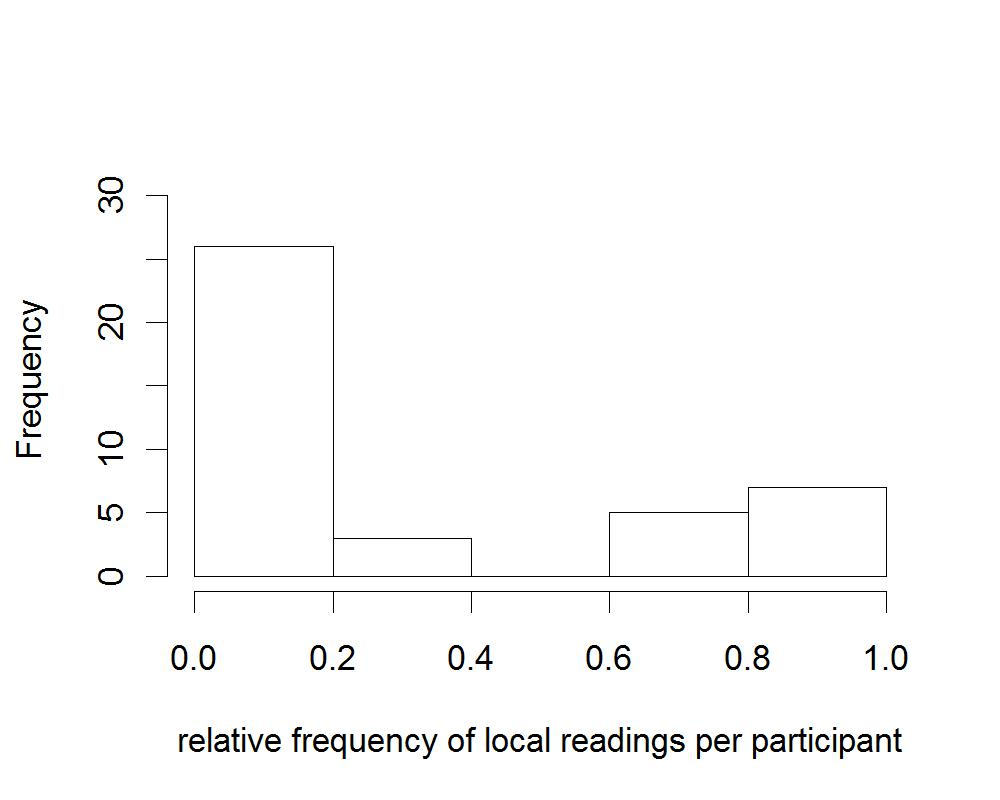
\includegraphics[width=5cm]{histLocalReadingGE_NTR.jpg}
\label{fig:ReadingsGE}
}
\label{fig:HistogramLocalReadingsK2}
\caption[Optional caption for list of figures]{Judgments for the four target conditions}
\end{figure}



\bibliography{../../Literatur/tex/literatur}
\end{document}
